\documentclass[twocolumn,letterpaper,10pt]{article}
\usepackage[utf8]{inputenc}
\usepackage{times}
\usepackage{helvet}
\usepackage{courier}
\usepackage{txfonts}
\usepackage{subcaption}
\frenchspacing
%\setlength{\pdfpagewidth}{8.5in}
%\setlength{\pdfpageheight}{11in}

%used for pseudocode
\usepackage{algpseudocode}

%used to make charts
\usepackage{pgfplotstable}
\usepackage{pgfplots}

%used for mathematical notation
\usepackage{amsfonts}

%used to control spacing in table captions
\usepackage{subfig}

%used to import images
\usepackage{graphicx}

%used to specify table placement
\usepackage{float}

% Make it so lists don't have extra line spacing:
\usepackage{enumitem}
\setlist{noitemsep}

\usepackage{hyperref} % for \url

% For nice, customizable code listings:
\usepackage{listings}
\lstset{ %http://stackoverflow.com/questions/586572/make-code-in-latex-look-nice
	language=Java,
	basicstyle=\footnotesize,       % font size
	numbers=left,                      % where line numbers appear
	numberstyle=\footnotesize,   % size of line numbers
	stepnumber=1,                    % how often line numbers appear
	numbersep=5pt,                   % space between line numbers and code
	showstringspaces=false,       % whether or not to show a _ in strings
	frame=single,                       % what kind of frame should be around the code
	xleftmargin=1.5em,
	xrightmargin=1em,
	framexleftmargin=0em,
	%rulecolor=\color{black},         % for the frame
	tabsize=2,                             % set the number of spaces for tabs
	breaklines=true,                     % set whether or not linebreaking should occur
	breakatwhitespace=true,          % set whether or not linebreaking should occur only at spaces
	lineskip={-1.0pt}
	%commentstyle=\color{mygreen}, % color for code comments
	%numberstyle=\color{mygray}, % style for line numbers
}


\renewcommand{\today}{}

\usepackage{plain} % for the bibliography

\title{Mask Recognition by Neural Networks}
\author{Aaryan Jha, Joel Magnabosco \\
\\ 
CSC 396: Research of Deep Neural Networks\\
Professor Bogaerts\\
Greencastle, IN, 46135, U.S.A.\\
}
\date{January 26 2023}

\begin{document}

\maketitle

\begin{abstract}
Masks are a major public health tool not only used for pandemic viruses, but are also used in everyday scenarios to still mitigate common viruses. Since the wake of COVID-19, monitoring and bolstering public health has had heightened importance. Mask detection is a great application of a deep neural network's capabilities, and is adaptive to tomorrow. After building 4 models to experiment on, 91\% testing accuracy was achieved. Our results show that dropout regularization is effective, and multiple convolution layers increases performance.
\end{abstract}

\section{Introduction}
\label{intro}
A mask detection program has many applications in our evolving world as governments still wrangle with COVID-19 issues, and health facilities still have mask requirements. Public surveillance continues to grow, and mask detection provides an extra edge for these tools. To train our neural network we used the mask detection data set from Kaggle authored by Omkar Gurav\cite{kaggle}. It consists of 7,553 images of people either wearing a mask or not. These images are then fed into a number of convolution layers depending on the model. The first layer applies 32 filters, the second applies 64 filters, third layer applies 128 filters, and the fourth applies 256 filters. All layers use the {\it ReLU} activation function. Followed by a max pooling layer with a filter shape of (2,2) and a stride of 2. Then each layer has a dropout probability that drops certain units out during training to force other units to train. The output of the last convolution layer is the input for the first dense fully connected layer of 128 units. The remaining layer is the output layer with only 2 units. Below is Figure \ref{fig:net}, showing a diagram of the basic structure of the neural network that makes up the experimental models. 

\begin{figure}[!h]
\begin{center}
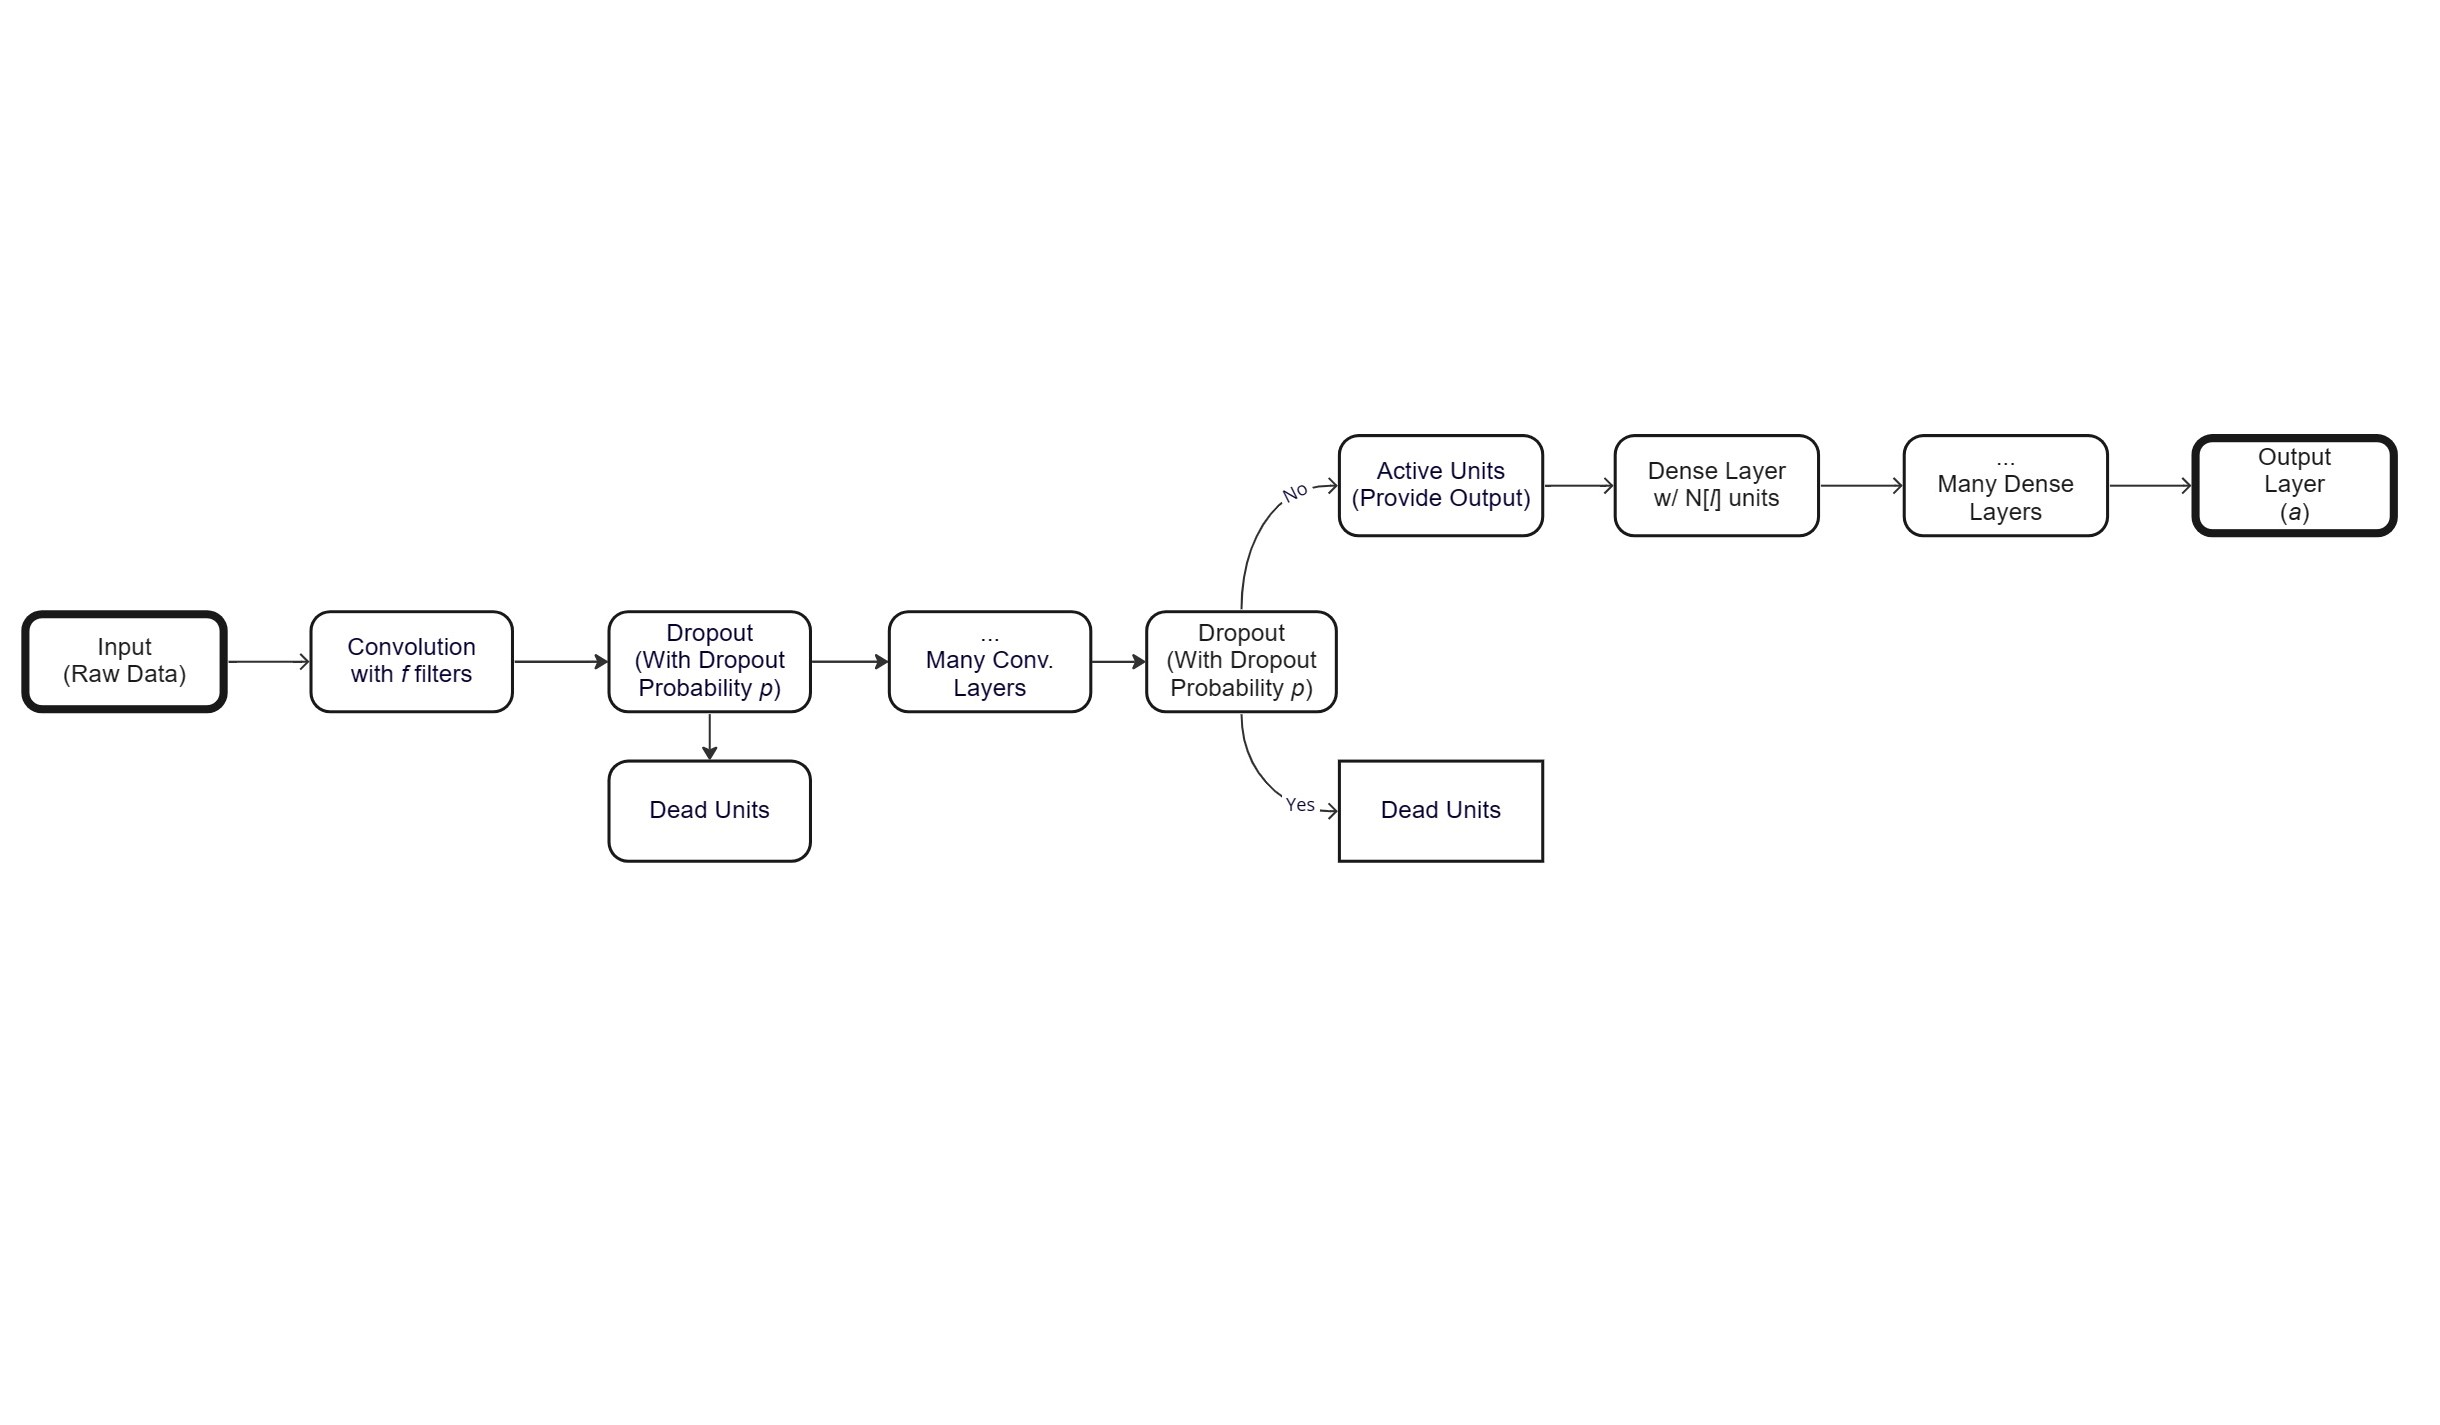
\includegraphics[width=.95\linewidth,height=2.5in]{networkDiagram.jpg}
\end{center}
\caption{Simplified structure of a basic neural network}
\label{fig:net}
\end{figure}

Bellow is a brief explanation of the algorithms employed in these models, and some of the methodology behind the network found in framework section \ref{frame}. Followed by the experimental set-up \ref{setup} providing an explanation of our experimentation, and details about each model being ran. the results section \ref{results} provides accuracy numbers with some graphs, and the analysis section \ref{analysis} adds meaning and context to these numbers.\\ 


\section{Framework}
\label{frame} 
Dropout regularization uses a dropout probability to "deaden" units by zeroing their activation function. This is only done during training to improve the training of the neural network. By doing so, the model generalizes better, and a higher test accuracy is achieved. Zeroing the activation function through the dropout probability forces the network to train on various units, and prevent over fitting during training. Of course during run time all units are active as desired. Dropout is applied for each layer of convolution and before inputs are passed to the dense layers.\\

The goal of an optimizer is to control the changes that are being made to the parameters in the network. In a way, dropout attempts to indirectly control weight values by dropping units out during training. The intuition behind RMSprop or root mean square propagation is that these parameters can't be large changes during training, because functions become much more complex and non-linear. By squaring these weights, units with large changes are lessened, and produce smoother training for the model. While the adam optimizer or adaptive moment estimation utilizes RMSprop, but also includes momentum and bias correction when making changes to the parameters. It uses corrected values to then calculate the changes made to the parameters.\\

The rectified linear units activation function or ReLU is used as the activation function for all the units in the models. ReLU simply returns only the positive values of x, and for negative values it produces zero. ReLU being a simple function bodes well for training to help minimize training error. The linearity of this function also keeps the hypothesis space simple for the neural network.\\

The dense layers consisting of 128 units in one and 2 in the other are the last layers of the neural network. These dense layers are ultimately what produces the output of the whole neural network. The weights from the last layer of convolution are then passed into the dense layers. Where they are multiplied with the biases at each unit. The formula below shows how an output is produced from multiple dense layers. 
$$
a^L = f(W^L * f(W^{L-1} * ... * f(W^2 * f(W^1 * x + b^1) + b^2) ... ) + b^L)
$$

\section{Experimental Set-up} 
\label{setup}

Our experiment consists of training and testing 4 different models with various different attributes to compare their performance on the classification of mask wearing. Our models are designed to focus in on  different aspects of neural network design. We are comparing convolution layer number, dropout probability, and two optimizers, {\it adam} and {\it RMSprop}. All models have 2 dense layers with 128 units in the first, and the second is the output layer with 2 units.The {\it ReLU} activation function is used for all convolution and dense layers.\\

Some of the various factors being tested all consists of two states. The convolution layers consist of a varying number. Either a single convolution layer applying 32 filters, two layers applying 32 and 64 filters respectively, or three layers with 32, 64, and 128 filters applied. The dropout probability being applied to these models are 0.0, 0.05, 0.1, and 0.2. Along with the two optimizers mentioned above.

\begin{itemize}
        \item Model 1 has a single convolution layer with zero dropout and the adam optimizer.
        \item Model 2 has two convolution layers with 0.05 dropout probability and the adam            optimizer.
        \item Model 3 has a single convolution layer with zero dropout and the RMSprop optimizer.
        \item Model 4 has two convolution layers with 0.05 dropout probability and the RMSprop optimizer.
\end{itemize}

Another batch of 6 models were constructed, and also ran with the following details. 
\begin{itemize}
        \item Model 5 has a single convolution layer, without dropout and the adam optimizer
        \item Model 6 has two convolution layers, with 0.1 dropout probaility, and the adam optimizer. 
        \item Model 7 has 3 convolution layers, with 0.2 dropout probability, and the adam optimizer.
        \item Model 8 has a single convolution layer, without dropout, and the RMSprop optimizer
        \item Model 9 has two convolution layers, with 0.1 dropout probability, and the RMSprop optimizer.
        \item Model 10 has three convolution layer, with 0.2 dropout probability, and the RMSprop optimizer.
\end{itemize}

\section{Results}
\label{results}
After training each model for 10 epochs, and testing the network with the testing set results were plotted. Testing accuracy plot along with validation accuracy are in figure \ref{fig:test} and in figure \ref{fig:val} below. Model  had the highest test accuracy at approximately 91.5\%. Model 4 also finished with the highest validation accuracy at epoch 10, but displayed a dramatic drop in validation accuracy early in the epochs. The lowest test accuracy was roughly 88.5\% produced by model 1. There isn't any real change in the validation plot in figure \ref{fig:val} after around 6 epochs. No signs of over fitting occur in the model besides the surprising result by model 4 in epoch three. A possible factor is a certain unit the network relied heavily on was dropped out causing the validation accuracy to take a dip. It's immediate return to the same levels as before within the next epoch suggests this. 

\begin{figure}[!h]

\begin{subfigure}{0.5\textwidth}
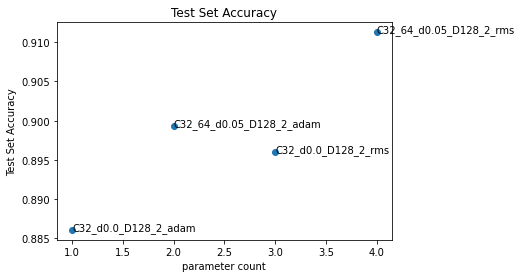
\includegraphics[width=0.9\linewidth, height=6cm]{Test_full.png} 
\caption{Test Accuracy for Models 1-4}
\label{fig:test}
\end{subfigure}
\begin{subfigure}{0.5\textwidth}
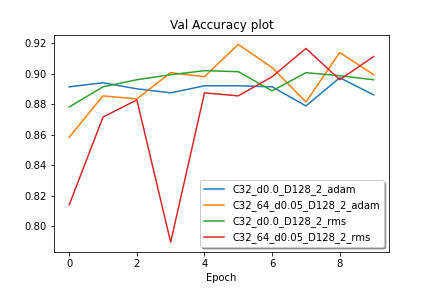
\includegraphics[width=0.9\linewidth, height=6cm]{Figure 1 - Validation Plot 1.png}
\caption{Validation Accuracy for Models 1-4}
\label{fig:val}
\end{subfigure}

\caption{Test and validation Accuracy for Models 1-4}
\label{fig:a}
\end{figure}

The test accuracy plots for the second batch of models is provided below in figure \ref{fig:b}. The RMSprop models (models 5-7) had it's highest test accuracy at roughly 95.5\%, while the adam models (models 8-10) topped out at 95.0\%. Both had a low at around 90\% testing accuracy, with two of the RMSprop models producing similarly low results near that 90\% low. The validation accuracy plots for these models is in figure \ref{fig:c} as well. Both validation accuracy plots look similar, with slightly more bounce in the RMSprop models, specifically model 9 in the eighth epoch. Both both groups of models achieve a similar high of 95\% and a low just shy of 90\%. 

\begin{figure}[!h]
\begin{subfigure}{0.5\textwidth}
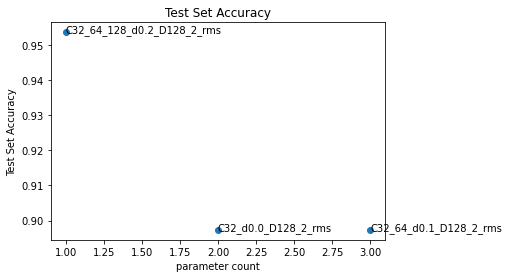
\includegraphics[width=0.9\linewidth, height=6cm]{rms_test_full.png} 
\caption{Test Accuracy for Models 5-7}
\label{fig:rmstest}
\end{subfigure}
\begin{subfigure}{0.5\textwidth}
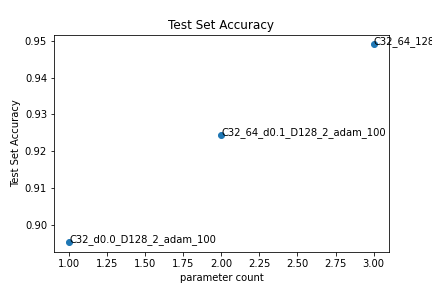
\includegraphics[width=0.9\linewidth, height=6cm]{test adam.png}
\caption{Test Accuracy for model 8-10}
\label{fig:adamtest}
\end{subfigure}

\caption{Results of the Test Accuracy for Models 5-10}
\label{fig:b}
\end{figure}

\section{Analysis}
\label{analysis}
Adding dropout to the convolutions layers is very effective at increasing the accuracy of a neural network. As seen in figure \ref{fig:test}, both models with dropout preformed better than the other two models with no dropout. Different convolution layer structures also had a similar result. Both models with only one convolution layer preformed worse than the other two models with 2 convolution layers. The highest testing accuracy for the single convolution layer models is roughly 89.5\%, while the lowest test accuracy for 2 layer models is approximately 90\%. The RMSprop optimizer performed better than the adam optimizer for each set of models they were compared against. The RMSprop optimizer produced higher testing accuracy for both dropout probability, and the number of convolution layers. However, in figure \ref{b} we can see that the adam optimizer does work better on the 2 layer network with 0.1 dropout probability.\\

As mentioned in section \ref{results}, Model 4 has a massive drop in validation accuracy around epoch 3. Dropout certainly adds noise to the lines in figure \ref{fig:val} with models 1 and 3 not nearly having as much volatility. These models also start with higher validation accuracy as a result of dropout being applied to the others. Although there is a slight decrease in validation accuracy for all of the models except model 4, the validation accuracy doesn't continue to worsen. By the tenth epoch, the validation accuracy is more or less similar to the accuracy before the sixth epoch for models. In terms of validation accuracy, both of the models with 2 convolution layers and dropout performed better than the smaller models. This is proof that applying dropout is working as intended to regularize the network and improving generalization by producing a higher validation accuracy. However, dropout doesn't guarantee better performance seen by model 9 in figure \ref{fig:rmstest} where including dropout didn't increase accuracy. While in figure \ref{fig:adamtest} there are obvious levels of improvement. The 90\% testing accuracy is also important to note, because there are only two classifications so returning the same result only yields a 50\% accuracy. 

\section{Future Work}
\label{future}
More is needed to improve this neural network, and for it to be implemented on a daily use basis. More layers of convolution could be tested to see the effect if it has on performance. Only two convolution layers brings a considerable boost to accuracy. Three layers of convolution preformed even better. Considering that the RMSprop optimizer performed better than the adam optimizer, the RMSprop optimizer can be used to continue the experimentation of this neural network. However, the drop in performance of model 4 in figure \ref{fig:val}, and the drop in performance of model 9 in figure\ref{fig:rmsval} suggest that RMSprop isn't as smooth as the adam poptimizer. Our experiment proves that dropout is effective for regularization, and possibly higher levels of dropout could be tested for increased performance. 


\section{Conclusion}
Neural networks are full of potential as the learning capabilities of these models improves, and it's ability to adapt to applications, like mask detection in our case. Through the power of convolution layers and dense layers, a model can be created that can classify really well. We explored the various structures that could be implemented in achieving the problem of mask detection by changing the number of convolution layers, the dropout probability, and the optimizer used in each model. The models constructed were able to achieve high levels of accuracy around 95\%. Our experimentation demonstrated the usefulness of dropout for regularization illustrated by higher validation and testing accuracy values. More than a singular convolution layer should be used for a network like this, as adding a second layer consistently increased accuracy. The comparison between the RMSprop and adam optimizers is a cautionary tale, as the RMSprop optimizer produces better overall results. However, it lacks some consistency displayed in figure \ref{fig:rmstest}, and there also seems to be spots of inconsistency in both figures \ref{fig:val} and \ref{fig:rmsval}. For this model to properly be implemented in the real world, live video processing will need to be Incorporated into its capabilities. Furthermore, mask detection is a good demonstration of the capabilities of deep neural networks, and the task of mask detection provided a good measuring stick for the analysis of results.

\section{Appendix}
\label{append}

\begin{figure}[!h]
\begin{subfigure}{0.5\textwidth}
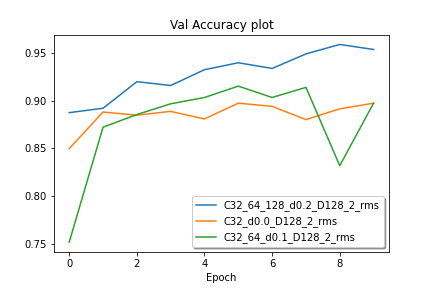
\includegraphics[width=0.9\linewidth, height=6cm]{Figure 3 - Validation Plot 1.png} 
\caption{Validation Accuracy for Models 5-7}
\label{fig:rmsval}
\end{subfigure}
\begin{subfigure}{0.5\textwidth}
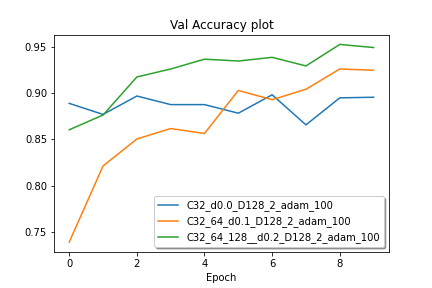
\includegraphics[width=0.9\linewidth, height=6cm]{val adam.png}
\caption{Validation Accuracy for model 8-10}
\label{fig:adamval}
\end{subfigure}

\caption{Results of the Validation Accuracy for Models 5-10}
\label{fig:c}
\end{figure}

\bibliographystyle{plain}
\bibliography{final}

\end{document}
